\documentclass[12pt]{article}
\usepackage[margin=0.3in,top=0.25in,bottom=0.4in]{geometry}
\makeatletter
\renewcommand{\@maketitle}{\newpage\null\vskip -3.5em\begin{center}{\LARGE \@title \par}\end{center}\par\vskip 0.2em}
\makeatother
\usepackage{amsmath,amssymb}
\usepackage{booktabs}
\usepackage{graphicx}
\usepackage{hyperref}
\setlength{\parskip}{0.6em}
\setlength{\parindent}{0pt}
\newcommand{\xpo}{x_{\mathbb{P}}}

\title{Large-$P_\perp$ tail of the exclusive cross section}
\author{}
\date{}

\begin{document}
\sloppy
\maketitle

\section*{In short}

The notes on the large-$P_\perp$ behaviour (Sec.~4 and Erratum) predict, at fixed $z$ and $\xpo$:
GBW $\Rightarrow m^2Q_s^4/P_\perp^8$; MV $\Rightarrow Q_s^4/P_\perp^6$, from the logarithm in
$\mathcal{N}\sim Q_s^2r_\perp^2\ln(1/r_\perp\Lambda)$. Both are confirmed numerically (Fig.~\ref{fig:tail}).
Our dipole, however, is the MVe fit with $e_c=18.9$ inside the logarithm. This delays the
$1/P_\perp^6$ tail to $P_\perp\gtrsim50$~GeV; below it the spectrum behaves almost like GBW:
\begin{itemize}
\item MVe at fixed $\xpo$: local power $-6.9$ at 5~GeV, $-7.4$ at 10~GeV, $-7.0$ at 20~GeV, $-6.1$ at
  50~GeV, $\to-6$ above 100~GeV. BK evolution makes it flatter: $-6.9$ ($x=10^{-3}$) and $-6.0$
  ($x=10^{-5}$) at 10~GeV.
\item The code at fixed $q^+=2p^+$ falls as $P_\perp^{-8.5}$ at 12--20~GeV. This is the fixed-$\xpo$ power
  ($\approx-7.2$) plus $\approx-1.3$ from $\xpo=M^2/W^2\propto m_T$, which grows with $P_\perp$ and lowers
  $Q_s$. The code's radial integrals agree with an independent evaluation to $10^{-4}$.
\item So the $1/P_\perp^6$ tail is correct for MV, but it is not reached in our $p_\perp$ range: there is
  nothing wrong with the steeper fall of our exclusive results.
\end{itemize}

\section*{1. Formulae}

Exclusive $c\bar c$ photoproduction ($Q^2=0$, $\bar Q^2=m^2$) at fixed $z$, Eq.~(4.2) of the notes:
\begin{equation}
\frac{\mathrm{d}\sigma}{\mathrm{d}^2P_\perp\mathrm{d}z}=\frac{\alpha_{\mathrm{em}}e_q^2N_cS_\perp}{2\pi^2}\,F(P_\perp)\,,\qquad
F=m^2\Big[(z^2+\bar z^2)\,I_1^2+I_0^2\Big],\qquad
I_\nu=\int_0^\infty\!\mathrm{d}r\,r\,J_\nu(P_\perp r)K_\nu(mr)\,\mathcal{N}(r)\,.
\end{equation}
We take $z=\tfrac12$, $m=1.5$~GeV. The code (\texttt{exclusiveCrossSection\_fixed\_qp}) returns
$z\,m^2[(z^2+\bar z^2)I_1^2+I_0^2]=F/2$ at $z=\tfrac12$, with $\xpo=M_{q\bar q}^2/W^2$, $W^2=2m_Te^y\sqrt s$.

Dipole amplitudes ($Q_{s0}^2=0.06$~GeV$^2$, $\Lambda=0.241$~GeV, header of \texttt{data/proton/mve.dat}):
\begin{align}
\text{MVe:}\quad&\mathcal{N}(r)=1-\exp\Big[-\frac{r^2Q_{s0}^2}{4}\ln\Big(\frac{1}{r\Lambda}+e_c\,e\Big)\Big],\quad e_c=18.9\,,\\
\text{MV:}\quad&\text{the same with }e_c=1\,,\\
\text{GBW:}\quad&\mathcal{N}(r)=1-\exp\Big[-\frac{r^2Q_{s0}^2}{4}\,L_0\Big],\quad L_0=\ln\Big(\frac{m}{\Lambda}+e_c\,e\Big)
\ \text{(the MVe log at $r=1/m$)}\,.
\end{align}
The BK solution of \texttt{mve.dat} starts from MVe at $x_0=0.01$.

\section*{2. Why $e_c$ delays the $1/P_\perp^6$ tail}

At large $P_\perp$, with $r=u/P_\perp$, only the small-$r$ form $\mathcal{N}\approx\frac{r^2Q_{s0}^2}{4}L(r)$ matters,
$L(r)=\ln(1/r\Lambda+e_c e)$. The transverse term is
\begin{equation}
I_1\approx\frac{Q_{s0}^2}{4mP_\perp^2}\int_0^\infty\!\mathrm{d}u\,u^2J_1(u)\,L(u/P_\perp)\,.
\end{equation}
A constant $L$ gives zero, since $\int\mathrm{d}u\,u^2J_1(u)=0$ (Eq.~(4.6) of the notes): that is the GBW
case, where only the mass term survives, $F\propto m^2Q_s^4/P_\perp^8$. The $1/P_\perp^6$ term comes from the
$u$ dependence of $L$, i.e.\ from
\begin{equation}
\frac{\mathrm{d}L}{\mathrm{d}\ln(1/r)}=\frac{1}{1+e_c e\,\Lambda r}=\frac{1}{1+e_c e\,\Lambda\,u/P_\perp}\,.
\end{equation}
For MV ($e_c=1$) this is $\approx1$ already for $P_\perp\gtrsim$ a few GeV, and with
$\int\mathrm{d}u\,u^2\ln(1/u)J_1(u)=2$ (Eq.~(4.17)) one gets $F\propto Q_s^4/P_\perp^6$, Eq.~(4.18). For MVe,
$e_c e\Lambda=12.4$~GeV, so the logarithm only starts to vary when $P_\perp\gtrsim12.4\,u$; with
$u\approx2$--4 in the integral, the $1/P_\perp^6$ term takes over only at $P_\perp\approx25$--50~GeV. Below it
MVe behaves like GBW with a slowly varying effective log.

\section*{3. Numerical check}

$I_0$ and $I_1$ are computed with Gauss--Legendre (24 points) between consecutive zeros of $J_\nu(P_\perp r)$,
up to $r=40$~GeV$^{-1}$ (\texttt{plotting\_scripts/exclusive\_tail.py}). The BK amplitude is interpolated
linearly in $y=\ln(x_0/x)$ between blocks, as in AmplitudeLib, and with a cubic spline in $(\ln r,\ln\mathcal{N})$.
Two checks:
\begin{itemize}
\item The BK file at $x=x_0$ reproduces the analytic MVe exactly (dashed and solid blue in Fig.~\ref{fig:tail}).
\item At $\xpo=M^2/W^2$ (frozen above 0.01) it reproduces the code's \texttt{output/charm/charm\_fixed\_qp\_y00.dat}
  to $10^{-4}$ at all 20 points from 2 to 20~GeV: the GSL integrals in the code are accurate.
  Here $x=\xpo(P_\perp)=2m_T/\sqrt s$ ($y=0$, $z=\tfrac12$):
  $0.9\times10^{-3}$ at 2~GeV, $2\times10^{-3}$ at 5~GeV, $3.8\times10^{-3}$ at 10~GeV, $7.5\times10^{-3}$ at
  20~GeV. So the dots start near the BK $x=10^{-3}$ line and move towards the MVe ($x=x_0$) line; they do
  not follow any fixed-$x$ line.
\end{itemize}
The figure stops at 100~GeV; the table in Sec.~4 gives the analytic models up to 1000~GeV. The evolved BK
curves are not extended beyond 100~GeV: there ($r\lesssim10^{-2}$~GeV$^{-1}$) their local power becomes
noisy, from the numerical BK solution.

\begin{figure}[h]
\centering
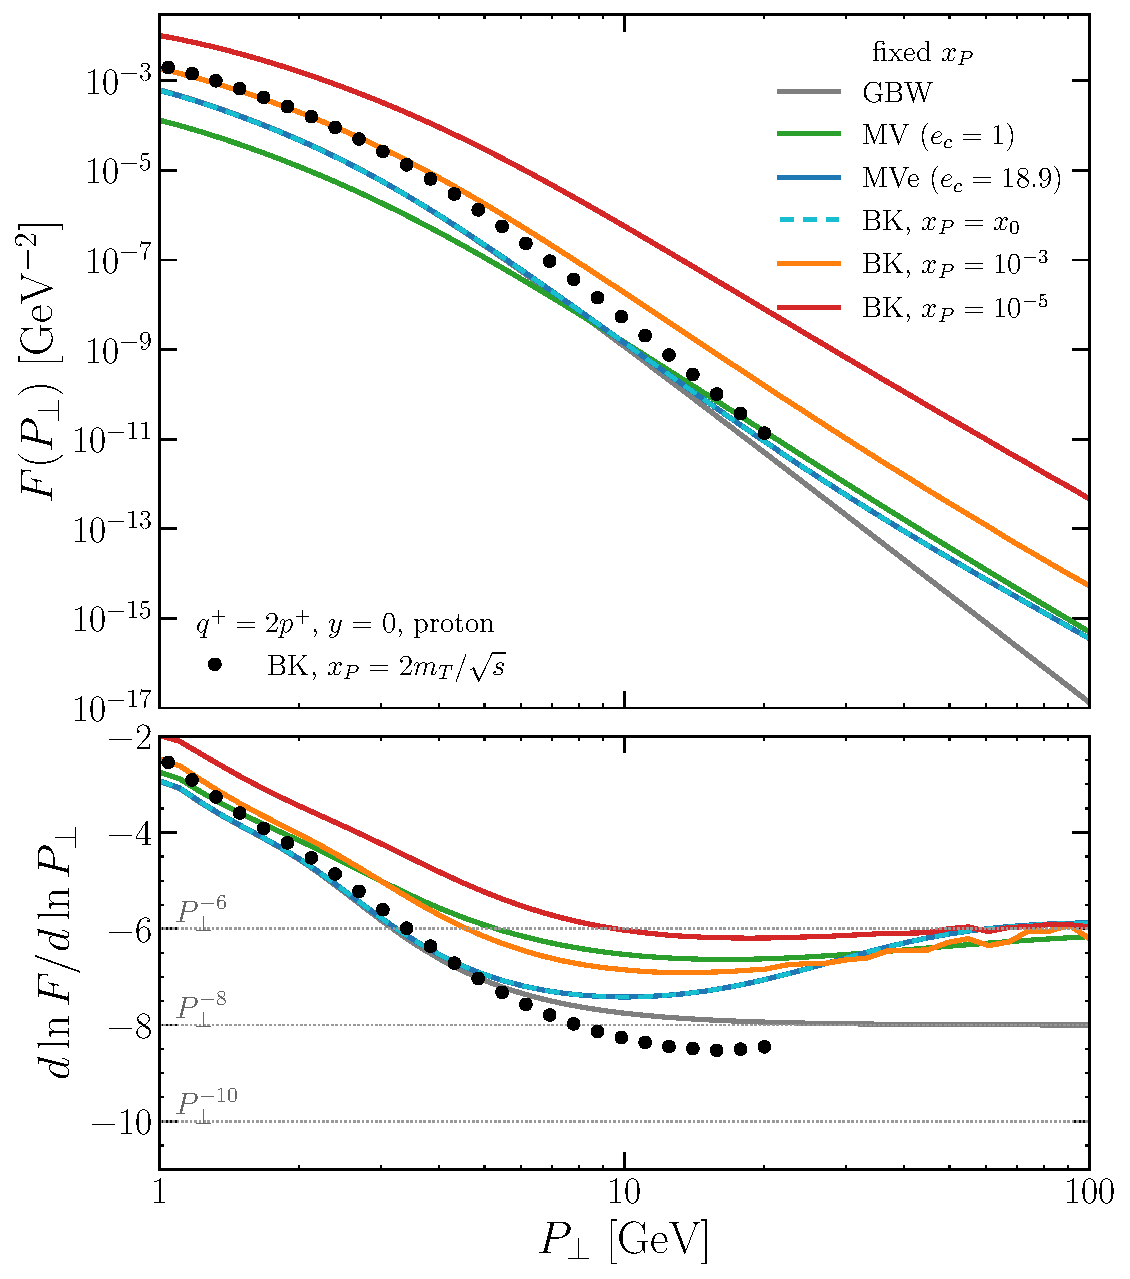
\includegraphics[width=0.62\textwidth]{../plots/exclusive_tail.pdf}
\caption{Top: $F(P_\perp)$ at $z=\tfrac12$ for GBW, MV, MVe and the BK solution at fixed $x$, and the code at
fixed $q^+=2p^+$ ($y=0$, proton) where $\xpo$ grows with $P_\perp$ (black dots). Bottom: local power
$\mathrm{d}\ln F/\mathrm{d}\ln P_\perp$; dotted lines at $-6$, $-8$, $-10$.}
\label{fig:tail}
\end{figure}

\subsection*{Reading the figure}

\textbf{What is plotted.} The top panel shows $F(P_\perp)=m^2[(z^2+\bar z^2)I_1^2+I_0^2]$, the exclusive cross section
$\mathrm{d}\sigma/\mathrm{d}^2P_\perp\mathrm{d}z$ at $z=\tfrac12$ without the constant prefactor
$\alpha_{\mathrm{em}}e_q^2N_cS_\perp/2\pi^2$; hence the units GeV$^{-2}$. There is no photon flux and no fragmentation:
it is the parton-level $c\bar c$ spectrum. The bottom panel shows its local power
$n(P_\perp)=\mathrm{d}\ln F/\mathrm{d}\ln P_\perp$, so that $F\propto P_\perp^{\,n}$ locally; a pure power law is a
horizontal line.

\textbf{The lines: one dipole amplitude at one fixed $x$ each.} Every line uses the same formula for $F$ and differs
only in $\mathcal N(r)$:
\begin{itemize}
\item GBW, MV and MVe are the analytic models of Sec.~1, with no $x$ dependence.
\item ``BK, $\xpo=x_0$'' is the BK solution of \texttt{mve.dat} at its initial condition. It lies exactly on MVe,
  which checks that the file is read correctly.
\item ``BK, $\xpo=10^{-3}$'' and ``BK, $\xpo=10^{-5}$'' are the same BK solution after evolution. Evolution raises $Q_s$, so
  $F$ is larger, and makes $\mathcal N$ at small $r$ closer to the MV form, so the tail is flatter.
\end{itemize}
Since $x$ is the same at all $P_\perp$ along a line, the lines isolate the $P_\perp$ dependence of the Hankel integrals
$I_0$, $I_1$. That dependence is what the notes compute, so the lines are the ones to compare with $P_\perp^{-6}$ and
$P_\perp^{-8}$.

\textbf{The dots: our exclusive result, where $\xpo$ changes with $P_\perp$.} The dots are the code output
\texttt{output/charm/charm\_fixed\_qp\_y00.dat} (times 2, since the code returns $F/2$). In the code the photon
energy is fixed by $q^+=2p^+$, so the energy of the $\gamma p$ system, $W^2=2m_Te^y\sqrt s$, and the invariant mass
of the pair, $M_{c\bar c}^2=m_T^2/z\bar z=4m_T^2$, both depend on $P_\perp$. The amplitude is evaluated at
\begin{equation}
\xpo=\frac{M_{c\bar c}^2}{W^2}=\frac{2m_T}{e^y\sqrt s}\,,
\end{equation}
which at $y=0$ rises from $0.9\times10^{-3}$ at 2~GeV to $7.5\times10^{-3}$ at 20~GeV. Each dot therefore belongs to a
different BK line:
\begin{itemize}
\item at 2~GeV it sits on the BK $x=10^{-3}$ line;
\item as $P_\perp$ grows, $\xpo$ grows, so $Q_s$ decreases and the dots drift down towards the MVe ($x=x_0$) line.
\end{itemize}
This drift is why the dots cross the fixed-$x$ lines and fall faster than any of them: $-8.5$ instead of $\approx-7$.
The extra $-1.3$ is the $\xpo$ dependence $F\propto\xpo^{-1.3}$ combined with $\xpo\propto m_T$ (Sec.~4).

Evaluating the BK solution at the dots' own $\xpo(P_\perp)$ reproduces every dot to $3\times10^{-5}$ from 2 to
20~GeV. So the dots and the BK lines do not disagree: they are the same amplitude, sampled along different paths in
$(P_\perp,x)$.

\textbf{Consequence for the $P_\perp^{-6}$ question.} The notes' $P_\perp^{-6}$ is a statement at fixed $x$: it is
the MV line, and it is reached by MVe only above $\approx50$~GeV (Sec.~2). Our spectrum is not at fixed $x$, and in
our range it is steeper for two separate reasons: the large $e_c$ of the fit, which keeps the fixed-$x$ power near
$-7$, and the growth of $\xpo$ with $P_\perp$, which adds $\approx-1.3$.

\section*{4. Local powers}

$\mathrm{d}\ln F/\mathrm{d}\ln P_\perp$:
\begin{center}
\begin{tabular}{l|ccccccc}
\toprule
$P_\perp$ [GeV] & 5 & 10 & 20 & 50 & 100 & 300 & 1000 \\
\midrule
GBW                 & $-7.1$ & $-7.8$ & $-7.9$ & $-8.0$ & $-8.0$ & $-8.0$ & $-8.0$ \\
MV ($e_c=1$)        & $-5.9$ & $-6.5$ & $-6.6$ & $-6.4$ & $-6.2$ & $-6.0$ & $-6.0$ \\
MVe ($e_c=18.9$)    & $-6.9$ & $-7.4$ & $-7.0$ & $-6.1$ & $-5.9$ & $-5.9$ & $-6.0$ \\
BK, $x=10^{-3}$     & $-6.2$ & $-6.9$ & $-6.8$ & $-6.3$ & $-6.2$ & -- & -- \\
BK, $x=10^{-5}$     & $-5.2$ & $-6.0$ & $-6.2$ & $-6.0$ & $-6.0$ & -- & -- \\
code, $q^+=2p^+$    & $-7.2$ & $-8.3$ & $-8.5$ & -- & -- & -- & -- \\
\bottomrule
\end{tabular}
\end{center}
GBW tends to $-8$ ($m\neq0$, Eq.~(4.10)) and MV to $-6$ (Eq.~(4.18)), as predicted. The MV curve
overshoots to $-6.6$ around 10--20~GeV before it settles, from the logarithmic corrections to the asymptotic form.

\textbf{The code at fixed $q^+$.} At $y=0$, $\xpo=2m_T/\sqrt s$ grows from $10^{-3}$ at 2~GeV to $7.5\times10^{-3}$
at 20~GeV. At fixed $P_\perp=15$~GeV, $F\propto\xpo^{-1.3}$ (from $Q_s(\xpo)$), and the fixed-$\xpo$ power at
$\xpo\approx5\times10^{-3}$ is $-7.2$. Together: $-7.2-1.3\approx-8.5$, as found. In the $D^0$ spectrum the
photon flux at the required photon energy and the fragmentation steepen it further, to the
$\approx p_\perp^{-9}$ found before at 6--10~GeV.

\section*{5. Why BK evolution flattens the tail}

At large $P_\perp$ only small dipoles, $r\sim3/P_\perp$, contribute. Write the amplitude there as
$\mathcal N\propto(r^2)^{\gamma_{\mathrm{eff}}}$, with $\gamma_{\mathrm{eff}}=\mathrm{d}\ln\mathcal N/\mathrm{d}\ln r^2$. The power of $F$
is set by how far $\gamma_{\mathrm{eff}}$ is from 1:
\begin{itemize}
\item $\gamma=1$ exactly (GBW, $\mathcal N\propto r^2$): the transverse integral vanishes, $\int\mathrm{d}u\,u^2J_1(u)=0$,
  and only the mass term remains: $P_\perp^{-8}$.
\item $\gamma=1$ up to a logarithm (MV, $\mathcal N\propto r^2\ln(1/r)$): the logarithm leaves a remainder: $P_\perp^{-6}$.
\item $\gamma<1$ ($\mathcal N\propto r^{2\gamma}$): $I_1\simeq\frac1m\int\mathrm{d}r\,J_1(P_\perp r)\,\mathcal N(r)\propto P_\perp^{-1-2\gamma}$
  no longer vanishes, and $F\sim P_\perp^{-2-4\gamma}$, flatter than $-6$.
\end{itemize}
This last estimate only gives the direction: $\gamma_{\mathrm{eff}}$ changes with $r$, and the mass term also
contributes. Measured at $r=3/P_\perp$:
\begin{center}
\begin{tabular}{l|cccc|c}
\toprule
$\gamma_{\mathrm{eff}}$ at $r=3/P_\perp$, $P_\perp$ [GeV] & 5 & 10 & 20 & 50 & $Q_s^2$ [GeV$^2$] \\
\midrule
MVe ($e_c=18.9$), BK at $x_0$ & 0.975 & 0.972 & 0.959 & 0.940 & 0.24 \\
MV ($e_c=1$)                  & 0.836 & 0.849 & 0.866 & 0.887 & 0.08 \\
BK, $\xpo=10^{-3}$            & 0.836 & 0.872 & 0.892 & 0.906 & 0.34 \\
BK, $\xpo=10^{-5}$            & 0.660 & 0.735 & 0.785 & 0.828 & 1.0 \\
\bottomrule
\end{tabular}
\end{center}
\begin{itemize}
\item MVe starts almost as pure $r^2$ ($\gamma_{\mathrm{eff}}\approx0.97$): the large $e_c$ freezes the logarithm (Sec.~2),
  so it behaves almost like GBW.
\item BK evolution makes $\mathcal N$ grow faster than $r^2$ below $r_s$: in the dilute region the linear (BFKL) part of
  BK gives $\mathcal N\propto(r^2Q_s^2)^{\gamma}$ with $\gamma\approx0.6$--0.7, the anomalous dimension of geometric scaling.
  Evolution builds its own $r$ dependence and erases what $e_c$ imposed on the initial condition. The longer the
  evolution, the closer $\gamma_{\mathrm{eff}}$ gets to that value: 0.84 at $\xpo=10^{-3}$ ($Y=\ln(x_0/\xpo)=2.3$),
  0.66 at $\xpo=10^{-5}$ ($Y=6.9$), at $P_\perp=5$~GeV.
\item The $P_\perp^{-6}$ term is then no longer suppressed and dominates from a few GeV: $-6.9$ at 10~GeV for
  $\xpo=10^{-3}$, and $-5.2$ at 5~GeV for $\xpo=10^{-5}$ (Sec.~4).
\item The scaling region extends below $r_s$ only by an amount that grows with $Y$. At smaller $r$ (larger $P_\perp$) the
  amplitude has not yet been reshaped and is closer to the initial form, so $\gamma_{\mathrm{eff}}$ rises with $P_\perp$
  and all curves tend to $\approx-6$.
\item Evolution also raises $Q_s$ (last column; $Q_s^2=2/r_s^2$), which is why the BK curves lie higher.
\end{itemize}

\section*{Files}
Figure: \texttt{plotting\_scripts/exclusive\_tail.py} $\to$ \texttt{plots/exclusive\_tail.pdf}.
Input: \texttt{data/proton/mve.dat}, \texttt{output/charm/charm\_fixed\_qp\_y00.dat}.
Formulae: \texttt{notes-large\_pt-exclusive.pdf}, Sec.~4 and Erratum.

\end{document}
